\chapter{The Initial Mass Function: Theory}
\label{ch:imf_th}

\marginnote{
\textbf{Suggested background reading:}
\begin{itemize}
\item \href{http://adsabs.harvard.edu/abs/2014arXiv1402.0867K}{Krumholz, M.~R. 2014, Phys.~Rep., 539, 49}, section 6 \nocite{krumholz14c}
\end{itemize}
\textbf{Suggested literature:}
\begin{itemize}
\item \href{http://adsabs.harvard.edu/abs/2012MNRAS.423.2037H}{Hopkins, 2012, MNRAS, 423, 2037} \nocite{hopkins12d}
\item \href{http://adsabs.harvard.edu/abs/2012ApJ...754...71K}{Krumholz et al., 2012, ApJ, 754, 71} \nocite{krumholz12b}
\end{itemize}
}

The previous chapter discussed observations of the initial mass function, both how they are made and what they tell us. We now turn to theoretical attempts to explain the IMF. As with theoretical models of the star formation rate, there is at present no completely satisfactory theory for the origin of the IMF, just different ideas that do better or worse at various aspects of the problem. To recall, the things we would really like to explain most are (1) the slope of the powerlaw at high masses, and (2) the location of the peak mass. We would also like to explain the little-to-zero variation in these quantities with galactic environment. Furthermore, we would like to explain the origin of the distribution of binary properties.

\section{The Powerlaw Tail}

We begin by considering the powerlaw tail at high masses, $dn/dm \propto m^{-\Gamma}$ with $\Gamma \approx 2.3$. There are two main classes of theories for how this powerlaw tail is set: competitive accretion and turbulence. Both are scale-free processes that could plausibly produce a powerlaw distribution of masses comparable to what is observed.

\subsection{Competitive Accretion}

One hypothesis for how to produce a powerlaw mass distribution is to consider what will happen in a region where a collection of small "seed" stars form, and then begin to accrete at a rate that is a function of their current mass. Quantitatively, and for simplicity, suppose that every star accretes at a rate proportional to some power of its current mass, i.e.,
\begin{equation}
\frac{dm}{dt} \propto m^\eta.
\end{equation}
If we start with a mass $m_0$ and accretion rate $\dot{m}_0$ at time $t_0$, this ODE is easy to solve for the mass at later times. We get
\begin{equation}
m(t) = m_0 \left\{
\begin{array}{ll}
[1 - (\eta-1)\tau]^{1/(1-\eta)}, & \eta \neq 1 \\
\exp(\tau), & \eta = 1
\end{array}
\right.,
\end{equation}
where $\tau = t / (m_0/\dot{m}_0)$ is the time measured in units of the initial mass-doubling time. The case for $\eta = 1$ is the usual exponential growth, and the case for $\eta > 1$ is even faster, running away to infinite mass in a finite amount of time $\tau = 1/(\eta-1)$.

Now suppose that we start with a collection of stars that all begin at mass $m_0$, but have slightly different values of $\tau$ at which they stop growing, corresponding either to growth stopping at different physical times from one star to another, to stars stopping at the same time but having slightly different initial accretion rates $\dot{m}_0$, or some combination of both. What will the mass distribution of the resulting population be? If $dn/d\tau$ is the distribution of stopping times, then we will have
\begin{equation}
\frac{dn}{dm} \propto \frac{dn/d\tau}{dm/d\tau} \propto m(\tau)^{-\eta} \frac{dn}{d\tau}.
\end{equation}
Thus the final distribution of masses will be a powerlaw in mass, with index $-\eta$, going from $m(\tau_{\rm min})$ to $m(\tau_{\rm max})$; a powerlaw distribution naturally results.

The index of this powerlaw will depend on the index of the accretion law, $\eta$. What should this be? In the case of a point mass accreting from a uniform, infinite medium at rest, the accretion rate onto a point mass was worked out by \citet{hoyle46a} and \citet{bondi52a}, and the problem is known as Bondi-Hoyle accretion. The accretion rate scales as $\dot{m} \propto m^2$, so if this process describes how stars form, then the expected mass distribution should follow $dn/dm\propto m^{-2}$, not so far from the actual slope of $-2.3$ that we observe. A number of authors have argued that this difference can be made up by considering the effects of a crowded environment, where the feeding regions of smaller stars get tidally truncated, and thus the growth law winds up begin somewhat steeper than $\dot{m}\propto m^2$.

\begin{marginfigure}
\includegraphics[width=\linewidth]{imf_bate09}
\caption[IMF in a competitive accretion simulation]{
\label{fig:imf_bate09}
The IMF measured in a simulation of the collapse of a 500 $M_\odot$ initially uniform density cloud \citep{bate09b}. The single-hatched histogram shows all objects in the simulation, while the double-hatched one shows objects that have stopped accreting.
}
\end{marginfigure}
This is an extremely simple model, requiring no physics but hydrodynamics and gravity, and thus it is easy to simulate. Simulations done based on this model do sometimes return a mass distribution that looks much like the IMF, as illustrated in Figure \ref{fig:imf_bate09}. However, this appears to depend on the choice of initial conditions. Generally speaking, one gets about the right IMF if one stars with something with a viral ratio $\alpha_{\rm vir} \sim 1$ and no initial density structure, just velocities. Simulations that start with either supervirial or sub-virial initial conditions, or that begin with turbulent density structures, do not appear to grow as predicted by competitive accretion (e.g., \citealt{clark08a}).

Another potential problem with this model is that it only seems to work in environments where there is no substantial feedback to drive the turbulence or eject the gas. In simulations where this is not true, there appears to be no competitive accretion. The key issue is that competitive accretion seems to require a global collapse where all the stars fall together into a region where they can compete, and this is hard to accomplish in the presence of feedback.

Yet a third potential issue is that this model has trouble making sense of the IMF peak, as we will discuss in Section \ref{sec:imfpeak}.

\subsection{Turbulent Fragmentation}

A second class of models for the origin of the powerlaw slope is based on the physics of turbulence. The first of these models was proposed by \citet{padoan97a}, and there have been numerous refinements since \citep[e.g.,][]{padoan02a, padoan07a, hennebelle08b, hennebelle09a, hopkins12e, hopkins12d}. The basic assumption in the turbulence models is that the process of shocks repeatedly passing through an isothermal medium leads to a broad range of density distributions, and that stars form wherever a local region happens to be pushed to the point where it becomes self-gravitating. We then proceed as follows. Suppose we consider the density field smoothed on some size scale $\ell$. The mass of an object of density $\rho$ in this smoothed field is
\begin{equation}
m \sim \rho \ell^3,
\end{equation}
and the total mass of objects with characteristic density between $\rho$ and $\rho+d\rho$ is
\begin{equation}
dM_{\rm tot} \sim \rho p(\rho) \,d\rho,
\end{equation}
where $p(\rho)$ is the density PDF. Then the total number of objects in the mass range from $m$ to $m+dm$ on size scale $\ell$ can be obtained just by dividing the total mass of objects at a given density by the mass per object, and integrating over the density PDF on that size scale
\begin{equation}
\frac{dn_\ell}{dm} = \frac{dM_{\rm tot}}{m} \sim  \ell^{-3} \int p(\rho) \,d\rho.
\end{equation}

Not all of these structures will be bound. To filter out the ones that are, we impose a density threshold, analogous to the one we used in computing the star formation rate in Section \ref{ssec:eff_th}.\footnote{Indeed, several of the models discussed there allow simultaneous computation of the star formation rate and the IMF.} We assert that an object will be bound only if its gravitational energy exceeds its kinetic energy, that is, only if the density exceeds a critical value given by
\begin{equation}
\frac{Gm^2}{\ell} \sim m \sigma(\ell)^2
\qquad\Longrightarrow\qquad
\rho_{\rm crit} \sim \frac{\sigma(\ell)^2}{G \ell^2},
\end{equation}
where $\sigma(\ell)$ is the velocity dispersion on size scale $\ell$, which we take from the linewidth-size relation, $\sigma(\ell) = c_s (\ell/\ell_s)^{1/2}$. Thus we have a critical density
\begin{equation}
\rho_{\rm crit} \sim \frac{c_s^2}{G \ell_s \ell},
\end{equation}
and this forms a lower limit on the integral.

There are two more steps in the argument. One is simple: just integrate over all length scales to get the total number of objects. That is,
\begin{equation}
\frac{dn}{dm} \propto \int \frac{dn_\ell}{dm} \, d\ell.
\end{equation}
The second is that we must know the functional form $p(\rho)$ for the smoothed density PDF. One can estimate this in a variety of ways, but to date no one has performed a fully rigorous calculation. For example, \citet{hopkins12e} assumes that the PDF is lognormal no matter what scale it is smoothed on, and all that changes as one alters the smoothing scale is the dispersion. He obtains this by setting the dispersion on some scale $\sigma_\ell$ equal to an integral over the dispersions on all smaller scales. In contrast, \citet{hennebelle08b, hennebelle09a} assume that the density power spectrum is a powerlaw, and derive the density PDF from that. These two assumptions yield similar but not identical results.

\begin{marginfigure}
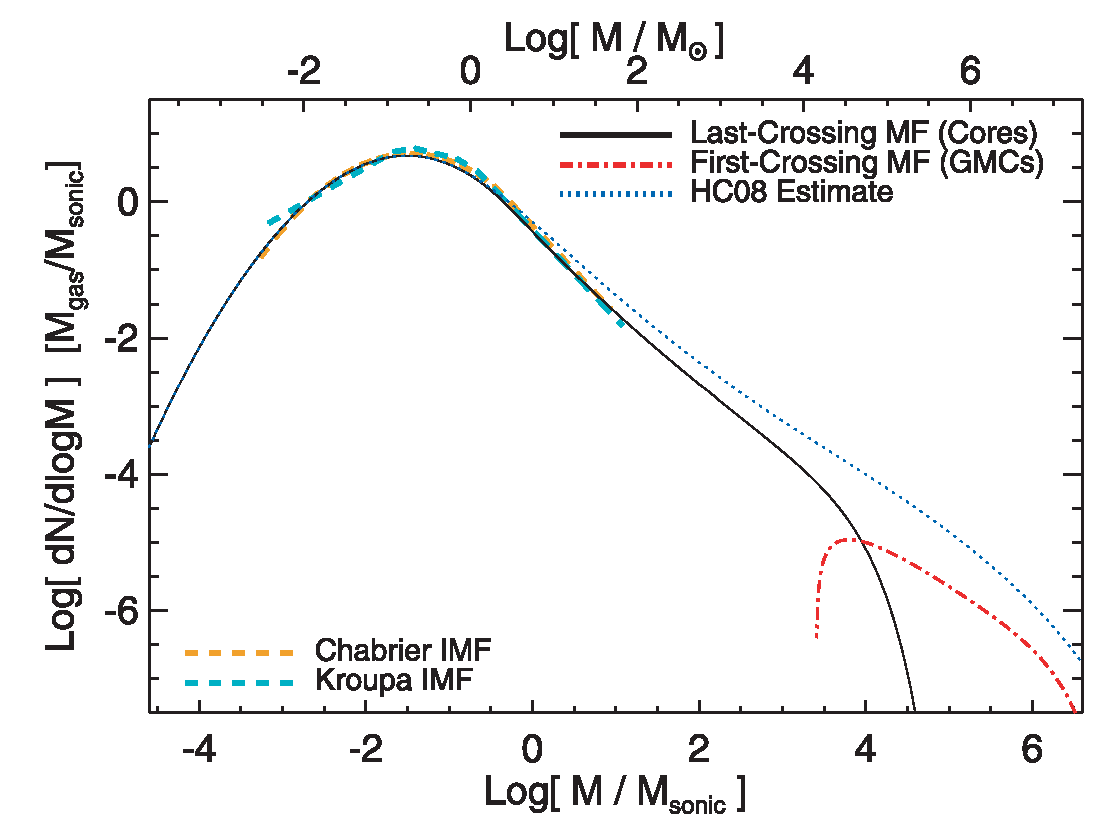
\includegraphics[width=\linewidth]{imf_hopkins12}
\caption[IMF from an analytic model of turbulent fragmentation]{
\label{fig:imf_hopkins12}
The IMF predicted by an analytic model of turbulent fragmentation by \citet{hopkins12d}.
}
\end{marginfigure}
At this point we will cease following the mathematical formalism in detail; interested readers can find it worked out in the papers referenced above. We will simply assert that one can at this point evaluate all the integrals to get an IMF. The result clearly depends only on two dimensional quantities: the sound speed $c_s$ and the sonic length $\ell_s$. However, at masses much greater than the sonic mass $M_s \approx c_s^2 \ell_s/G$, the result is close to a powerlaw with approximately the right index. Figure \ref{fig:imf_hopkins12} shows an example prediction.

As with the competitive accretion model, this hypothesis encounters certain difficulties. First, there is the technical problem that the choice of smoothed density PDF estimate is not at all rigorous, and there are noticeable differences in the result depending on how the choice is made. Second, the dependence on the sonic length is potentially problematic, because real molecular clouds do not have constant sonic lengths. Regions of massive star formation are observed to be systematically more turbulent. Third, the theory does not address the question of why gravitationally-bound regions do not sub-fragment as they collapse. Indeed, \citet{guszejnov15a} and \citet{guszejnov16a} argue that, when this effect is taken into account, the IMF (as opposed to the core mass distribution) becomes a pure powerlaw. As a result, the model has trouble explaining the IMF peak.

\section{The Peak of the IMF}
\label{sec:imfpeak}

\subsection{Basic Theoretical Considerations}

A powerlaw is scale-free, but the peak has a definite mass scale. This mass scale is one basic observable that any theory of star formation must be able to predict. Moreover, the presence of a characteristic mass scale immediately tells us something about the physical processes that must be involved in producing the IMF. We have thus far thought of molecular clouds as consisting mostly of isothermal, turbulent, magnetized, self-gravitating gas. However, we can show that there \textit{must} be additional processes beyond these at work in setting a peak mass.

We can see this in a few ways. First we can demonstrate it in a more intuitive but not rigorous manner, and then we can demonstrate it rigorously. The intuitive argument is as follows. In the system we have described, there are four energies in the problem: thermal energy, bulk kinetic energy, magnetic energy, and gravitational potential energy. From these energies we can define three dimensionless ratios, and the behavior of the system will be determined by these three ratios. As an example, we might define the Mach number, plasma beta, and Jeans number via
\begin{equation}
\mathcal{M} = \frac{\sigma}{c_s} \qquad \beta = \frac{8\pi \rho c_s^2}{B^2}
\qquad n_J = \frac{\rho L^2}{c_s^3/\sqrt{G^3\rho}}.
\end{equation}
The ratios describe the ratio of kinetic to thermal energy, the ratio of thermal to magnetic energy, and the ratio of thermal to gravitational energy. All other dimensionless numbers we normally use can be derived from these, e.g., the Alfv\'enic Mach number $\mathcal{M}_A = \mathcal{M}\sqrt{\beta/2}$ is simply the ratio of kinetic to magnetic energy.

Now notice the scalings of these numbers with density $\rho$, velocity dispersion $\sigma$, magnetic field strength $B$, and length scale $L$:
\begin{equation}
\mathcal{M} \propto \sigma
\qquad
\beta \propto \rho B^{-2}
\qquad
n_J \propto \rho^{3/2} L^3.
\end{equation}
If we scale the problem by $\rho\rightarrow x \rho$, $L\rightarrow x^{-1/2} L$, $B\rightarrow x^{1/2} B$, all of these dimensionless numbers remain fixed. Thus the behavior of two systems, one with density a factor of $x$ times larger than the other one, length a factor of $x^{-1/2}$ smaller, and magnetic field a factor of $x^{1/2}$ stronger, are simply rescaled versions of one another. If the first system fragments to make a star out of a certain part of its gas, the second system will too. Notice, however, that the {\it masses} of those stars will not be the same! The first star will have a mass that scales as $\rho L^3$, while the second will have a mass that scales as $(x\rho) (x^{-1/2} L)^3 = x^{-1/2} \rho L^3$. We learn from this an important lesson: isothermal gas is scale-free. If we have a model involving only isothermal gas with turbulence, gravity, and magnetic fields, and this model produces stars of a given mass $m_*$, then we can rescale the system to obtain an arbitrarily different mass.

Now that we understand the basic idea, we can show this a bit more formally. Consider the equations describing this system. For simplicity we will omit both viscosity and resistivity. These are
\begin{eqnarray}
\frac{\partial \rho}{\partial t} & = & -\nabla \cdot (\rho \vecv) \\
\frac{\partial}{\partial t}(\rho \vecv) & = & -\nabla \cdot (\rho\vecv\vecv) - c_s^2 \nabla \rho
\nonumber \\
& & {} + \frac{1}{4\pi} (\nabla \times \vecB) \times \vecB - \rho \nabla \phi \\
\frac{\partial\vecB}{\partial t} & = & -\nabla \times (\vecB\times\vecv) \\
\nabla^2 \phi & = & 4\pi G \rho
\end{eqnarray}
One can non-dimensionalize these equations by choosing a characteristic length scale $L$, velocity scale $V$, density scale $\rho_0$, and magnetic field scale $B_0$, and making a change of variables $\mathbf{x} = \mathbf{x}'L$, $t = t' L/V$, $\rho = r \rho_0$, $\mathbf{B} = \mathbf{b} B_0$, $\mathbf{v} = \mathbf{u} V$, and $\phi = \psi G\rho_0 L^2$. With fairly minimal algebra, the equations then reduce to
\begin{eqnarray}
\frac{\partial r}{\partial t'} & = & -\nabla'\cdot (r\mathbf{u}) \\
\frac{\partial}{\partial t'}(r \mathbf{u}) & = & -\nabla' \cdot \left(r\mathbf{uu}\right) - \frac{1}{\mathcal{M}^2}\nabla' r \nonumber \\
& & {} + \frac{1}{\mathcal{M}_A^2} (\nabla'\times\mathbf{b})\times\mathbf{b} - \frac{1}{\alpha_{\rm vir}} \nabla' \psi \\
\frac{\partial\mathbf{b}}{\partial t'} & = & -\nabla'\times\left(\mathbf{b}\times\mathbf{u}\right) \\
\nabla'^2 \psi & = & 4\pi r,
\end{eqnarray}
where $\nabla'$ indicates differentiation with respect to $x'$. The dimensionless ratios appearing in these equations are
\begin{eqnarray}
\mathcal{M} & = & \frac{V}{c_s} \\
\mathcal{M}_A & = & \frac{V}{V_A} = V\frac{\sqrt{4\pi \rho_0}}{B_0} \\
\alpha_{\rm vir} & = & \frac{V^2}{G \rho_0 L^2},
\end{eqnarray}
which are simply the Mach number, Alfv\'{e}n Mach number, and virial ratio for the system. These equations are fully identical to the original ones, so any solution to them is also a valid solution to the original equations. In particular, suppose we have a system of size scale $L$, density scale $\rho_0$, magnetic field scale $B_0$, velocity scale $V$, and sound speed $c_s$, and that the evolution of this system leads to a star-like object with a mass
\begin{equation}
m \propto \rho_0 L^3.
\end{equation}
One can immediately see that system with length scale $L' = y L$, density scale $\rho_0' = \rho_0 / y^2$, magnetic field scale $B_0' = B_0/y$, and velocity scale $V' = V$ has exactly the same values of $\mathcal{M}$, $\mathcal{M}_A$, and $\alpha_{\rm vir}$ as the original system, and therefore has exactly the same evolution. However, in this case the star-like object will instead have a mass
\begin{equation}
m' \propto \rho' L'^3 = y m
\end{equation}
Thus we can make objects of arbitrary mass just by rescaling the system.

This analysis implies that explaining the IMF peak requires appealing to some physics beyond that of isothermal, magnetized turbulence plus self-gravity. This immediately shows that the competitive accretion and turbulence theories we outlined to explain the powerlaw tail of the IMF cannot be adequate to explaining the IMF peak, at least not by themselves. Something must be added, and models for the origin of the IMF peak can be broadly classified based on what extra physics they choose to add.

\subsection{The IMF From Galactic Properties}

One option is hypothesize that the IMF is set at the outer scale of the turbulence, where the molecular clouds join to the atomic ISM (in a galaxy like the Milky Way), or on sizes of the galactic scale-height (for a molecule-dominated galaxy). Something in this outer scale picks out the characteristic mass of stars at the IMF peak.

This hypothesis comes in two flavors. The simplest is that characteristic mass is simply set by the Jeans mass at the mean density $\overline{\rho}$ of the cloud, so that
\begin{equation}
m_{\rm peak} \propto \frac{c_s^3}{\sqrt{G^3 \overline{\rho}}}
\end{equation}
While simple, this hypothesis immediately encounters problems. Molecular clouds have about the same temperature everywhere, but they do not all have the same density -- indeed, based on our result that the surface density is about constant, the density should vary with cloud mass as $M^{1/2}$. Thus at face value this hypothesis would seem to predict a factor of $\sim 3$ difference in characteristic peak mass between $10^4$ and $10^6$ $M_\odot$ clouds in the Milky Way. This is pretty hard to reconcile with observations. The problem is even worse if we think about other galaxies, where the range of density variation is much greater and thus the predicted IMF variation is too. One can hope for a convenient cancellation, whereby an increase in the density is balanced by an increase in temperature, but this seems to require a coincidence.

A somewhat more refined hypothesis, which is adopted by all the turbulence models, is that the IMF peak is set by the sound speed and the normalization of the linewidth-size relation. As discussed above, in the turbulence models the only dimensional free parameters are $c_s$ and $\ell_s$, and from them one can derive a mass in only one way:
\begin{equation}
m_{\rm peak} \sim \frac{c_s^2 \ell_s}{G}.
\end{equation}
\citet{hopkins12d} calls this quantity the sonic mass, but it's the same thing as the characteristic masses in the other models.

This value can be expressed in a few ways. Suppose that we have a cloud of characteristic mass $M$ and radius $R$. We can write the velocity dispersion in terms of the virial parameter:
\begin{equation}
\alpha_{\rm vir} \sim \frac{\sigma^2 R}{G M}
\qquad\Longrightarrow\qquad
\sigma \sim \sqrt{\alpha_{\rm vir} \frac{G M}{R}}.
\end{equation}
This is the velocity dispersion on the outer scale of the cloud, so we can also define the Mach number on this scale as
\begin{equation}
\mathcal{M} = \frac{\sigma}{c_s} \sim \sqrt{\alpha_{\rm vir} \frac{G M}{R c_s^2}}
\end{equation}
The sonic length is just the length scale at which $\mathcal{M} \sim 1$, so if the velocity dispersion scales with $\ell^{1/2}$, then we have
\begin{equation}
\ell_s \sim \frac{R}{\mathcal{M}^2} \sim \frac{c_s^2}{\alpha_{\rm vir} G \Sigma},
\end{equation}
where $\Sigma\sim M/R^2$ is the surface density. Substituting this in, we have
\begin{equation}
m_{\rm peak} \sim \frac{c_s^4}{\alpha_{\rm vir} G^2 \Sigma},
\end{equation}
and thus the peak mass simply depends on the surface density of the cloud. We can obtain another equivalent expression by noticing that
\begin{equation}
\frac{M_J}{\mathcal{M}} \sim \frac{c_s^3}{\sqrt{G^3 \overline{\rho}}} \sqrt{\frac{R c_s^2}{\alpha_{\rm vir} G M}}
\sim \frac{c_s^4}{\alpha_{\rm vir} G^2 \Sigma} \sim m_{\rm peak}
\end{equation}
Thus, up to a factor of order unity, this hypothesis is also equivalent to assuming that the characteristic mass is simply the Jeans mass divided by the Mach number.

An appealing aspect of this argument is that it naturally explains why molecular clouds in the Milky Way all make stars at about the same mass. A less appealing result is that it would seem to predict that the masses could be quite different in regions of different surface density, and we observe that there are star-forming regions where $\Sigma$ is indeed much higher than the mean of the Milky Way GMCs. This is doubly-true if we extend our range to extragalactic environments. One can hope that this will cancel because the temperature will be higher and thus $c_s$ will increase, but this again seems to depend on a lucky cancellation, and there is no \textit{a priori} reason why it should.

\subsection{Non-Isothermal Fragmentation}

The alternative to breaking the isothermality at the outer scale of the turbulence is to relax the assumption that the gas is isothermal on small scales. This has the advantage that it avoids any ambiguity about what constitutes the surface density or linewidth-size relation normalization for a "cloud".

\paragraph{Fixed equation of state models.}

\begin{marginfigure}
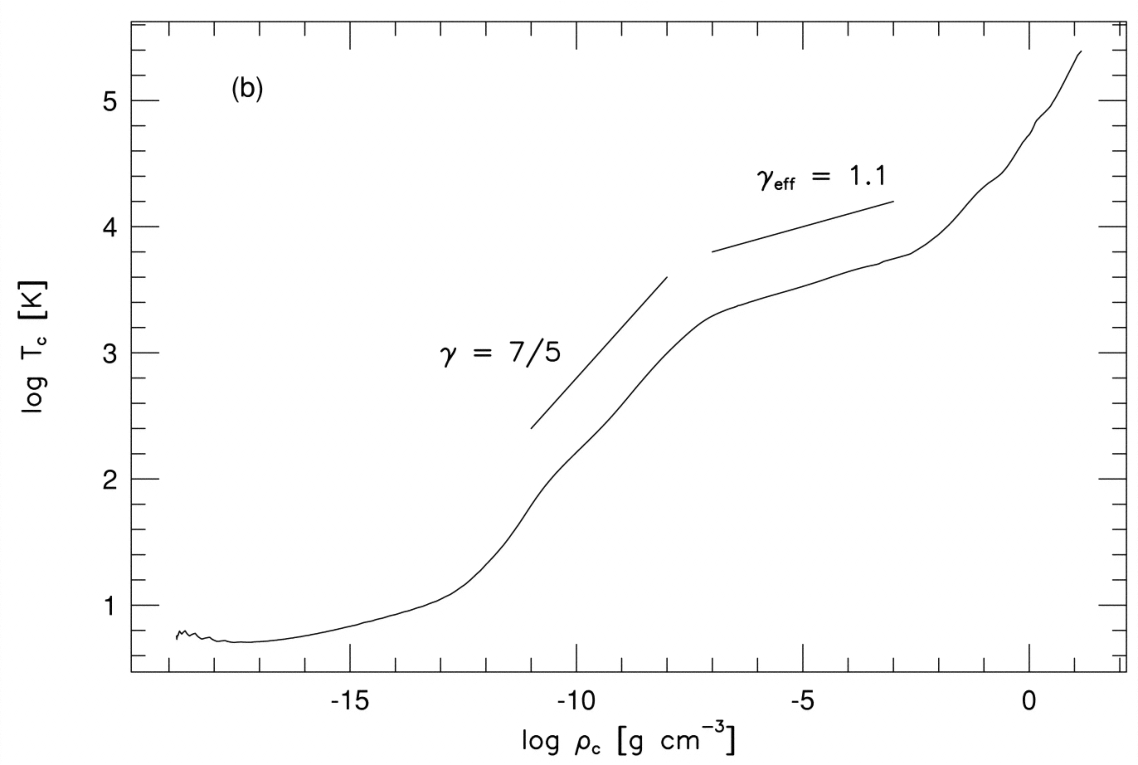
\includegraphics[width=\linewidth]{rhot_masunaga00}
\caption[Temperature versus density in a collapsing core]{
\label{fig:rhot_masunaga00}
Temperature versus density found in a one-dimensional calculation of the collapse of a $1$ $M_\odot$ gas cloud, at the moment immediately before a central protostar forms \citep{masunaga00a}.
}
\end{marginfigure}
The earliest versions of these models were proposed by \citet{larson05a}, and followed up by \citet{jappsen05a}. The basic idea of these models is that the gas in star-forming clouds is only approximately isothermal. Instead, there are small deviations from isothermality, which can pick out preferred mass scales. We will discuss these in more detail in Chapters \ref{ch:first_stars} and \ref{ch:protostar_form}, but for now we assert that there are two places where significant deviations from isothermality are expected (Figure \ref{fig:rhot_masunaga00}).

At low density the main heating source is cosmic rays and UV photons, both of which produce a constant heating rate per nucleus if attenuation is not significant. This is because the flux of CRs and UV photons is about constant, and the rate of energy deposition is just proportional to the number of target atoms or dust grains for them to interact with. Cooling is primarily by lines, either of CO once the gas is mostly molecular, or of C$^+$ or O where it is significantly atomic.

In both cases, at low density the gas is slightly below the critical density of the line, so the cooling rate per nucleus or per molecule is an increasing function of density. Since heating per nucleus is constant but cooling per nucleus increases, the equilibrium temperature decreases with density. As one goes to higher density and passes the CO critical density this effect ceases. At that point one generally starts to reach densities such that shielding against UV photons is significant, so the heating rate goes down and thus the temperature continues to drop with density.

This begins to change at a density of around $10^{-18}$ g cm$^{-3}$, $n\sim 10^5 - 10^6$ cm$^{-3}$. By this point the gas and dust have been thermally well-coupled by collisions, and the molecular lines are extremely optically thick, so dust is the main thermostat. As long as the gas is optically thin to thermal dust emission, which it is at these densities, the dust cooling rate per molecule is fixed, since the cooling rate just depends on the number of dust grains. Heating at these densities comes primarily from compression as the gas collapses, i.e., it is just $P\, dV$ work. If the compression were at a constant rate, the heating rate per molecule would be constant. However, the free-fall time decreases with density, so the collapse rate and thus the heating rate per molecule increase with density. The combination of fixed cooling rate and increasing heating rate causes the temperature to begin rising with density. At still higher densities, $\sim 10^{-13}$ g cm$^{-3}$, the gas becomes optically thick to dust thermal emission. At this point the gas simply acts adiabatically, with all the $P\,dV$ work being retained, so the heating rate with density rises again.

\citet{larson05a} pointed out that deviations from isothermality are particularly significant for filamentary structures, which dominate in turbulent flows.  It is possible to show that a filament cannot go into runaway collapse if $T$ varies with $\rho$ to a positive number, while it can collapse if $T$ varies as $\rho$ to a negative number. This suggests that filaments will collapse indefinitely in the low-density regime, but that their collapse will then halt around $10^{-18}$ g cm$^{-3}$, forcing them to break up into spheres in order to collapse further. The upshot of all these arguments is that the Jeans or Bonnor-Ebert mass one should be using to estimate the peak of the stellar mass spectrum is the one corresponding to the point where there is a changeover from sub-isothermal to super-isothermal.

In other words, the $\rho$ and $T$ that should be used to evaluate $M_J$ or $M_{\rm BE}$ are the values at that transition point. Larson proposes an approximate equation of state to represent the first break in the EOS:
Combining all these effects, \citet{larson05a} proposed a single simple equation of state
\begin{equation}
T = \left\{
\begin{array}{ll}
4.4 \,\rho_{18}^{-0.27}\mbox{ K}, \qquad & \rho_{18} < 1 \\
4.4 \,\rho_{18}^{0.07}\mbox{ K}, & \rho_{18} \ge 1
\end{array}
\right.
\end{equation}
where $\rho_{18}=\rho/(10^{-18}\mbox{ g cm}^{-3})$. Conveniently enough, the Bonnor-Ebert mass at the minimum temperature here is $M_{\rm BE} = 0.067$ $\msun$, which is not too far off from the observed peak of the IMF at $M=0.2$ $\msun$. (The mass at the second break is a bit less promising. At $\rho = 10^{-13}$ g cm$^{-3}$ and $T=10$ K, we have $M_{\rm BE} = 7\times 10^{-4}$ $\msun$.)

Simulations done adopting this proposed equation of state seem to verify the conjecture that the characteristic fragment mass does depend critically on the break on the EOS (Figure \ref{fig:imf_jappsen05}).

\begin{figure}
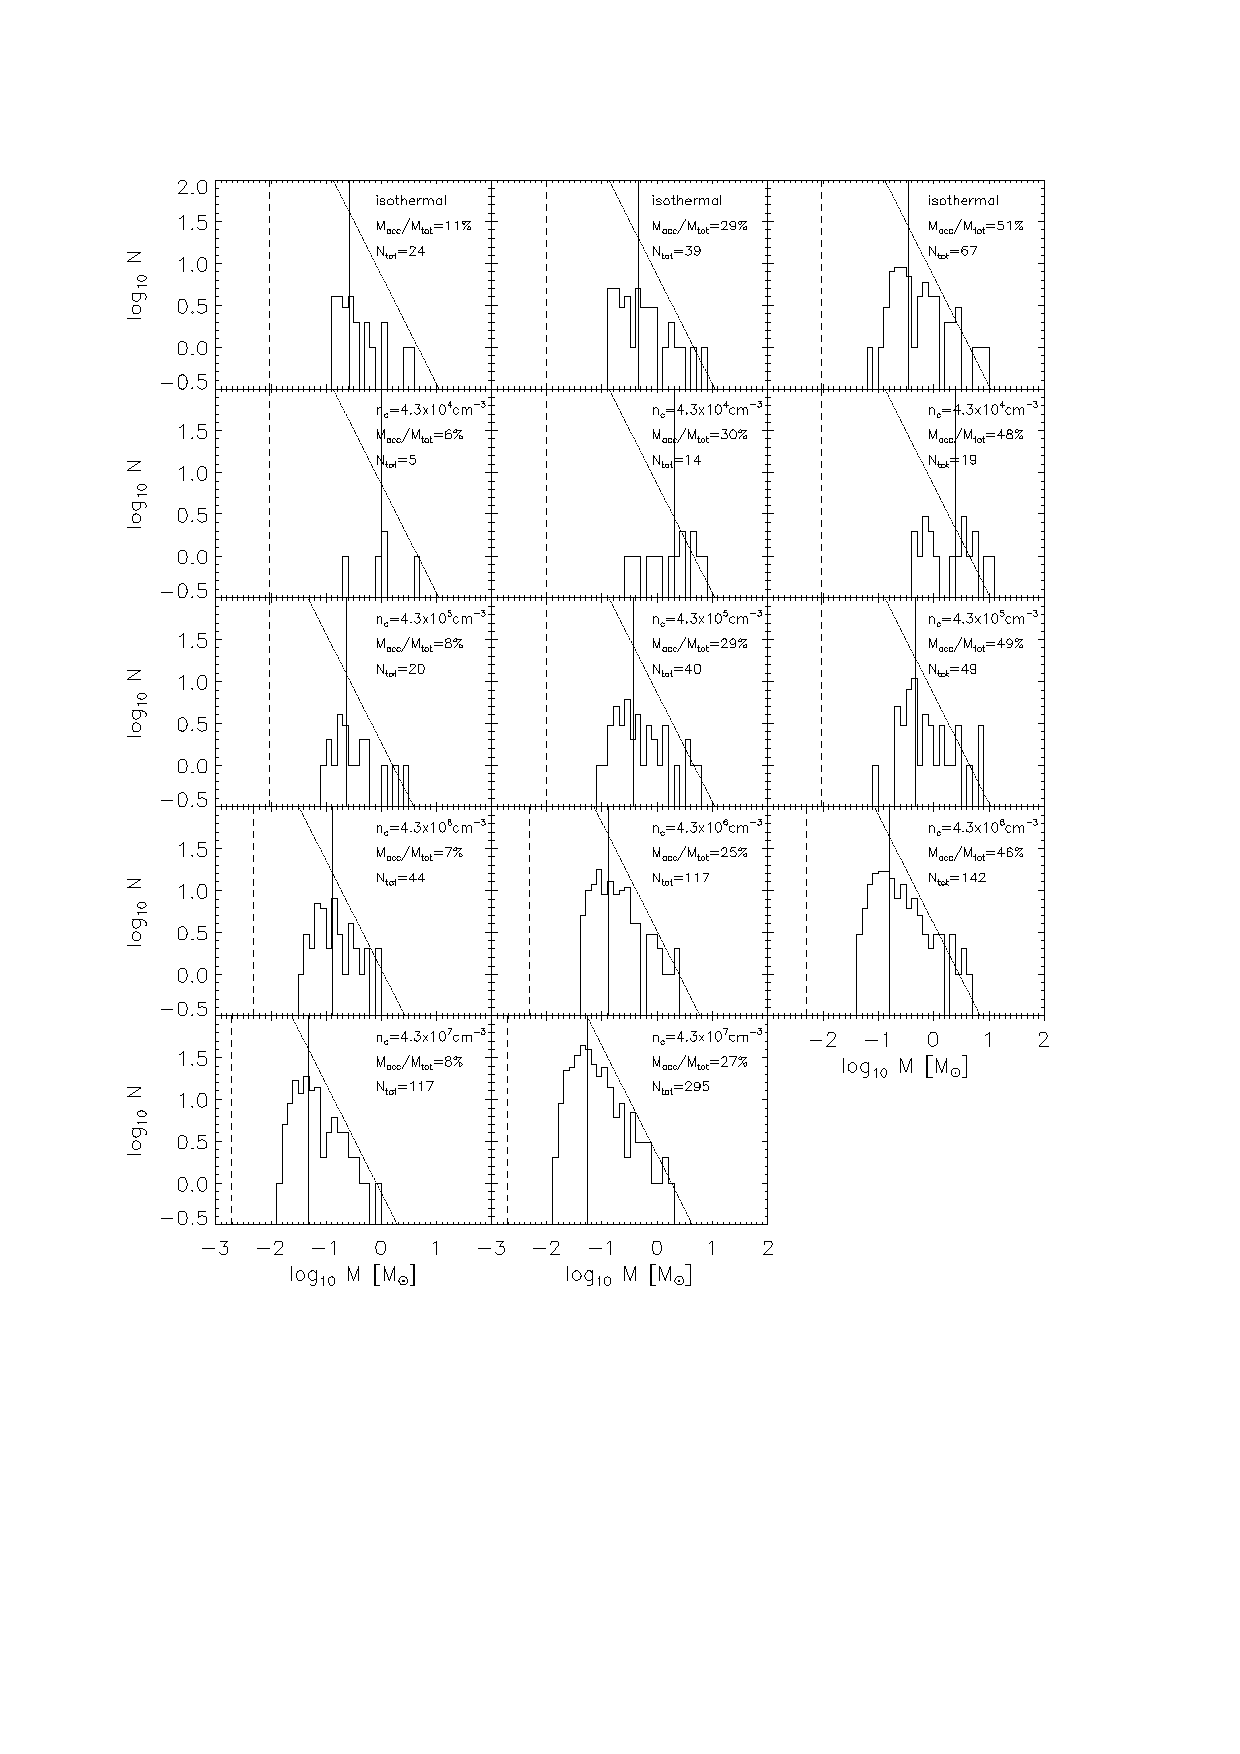
\includegraphics[width=\linewidth]{imf_jappsen05}
\caption[IMF from simulations of non-isothermal fragmentation]{
\label{fig:imf_jappsen05}
Measured stellar mass distributions in a series of simulations of turbulent fragmentation using non-isothermal equations of state. Each row shows a single simulation, measured at a series of times, characterized by a particular mass in stars as indicated in each panel. Different rows use different equations of state, with the vertical line in each panel indicating the Jeans mass evaluated at the temperature minimum of the equation of state. Histograms show the mass distributions measured for the stars.
}
\end{figure}

\paragraph{Radiative models.}

While this is a very interesting result, there are two problems. First, the proposed break in the EOS occurs at $n=4\times 10^5$ cm$^{-3}$. This is a fairly high density in a low mass star-forming region, but it is actually quite a low density in more typical, massive star-forming regions. For example, the Orion Nebula cluster now consists of $\approx 2000$ $\msun$ of stars in a radius of $0.8$ pc, giving a mean density $n\approx 2\times 10^4$ cm$^{-3}$. Since the star formation efficiency was less than unity and the cluster is probably expanding due to mass loss, the mean density was almost certainly higher while the stars were still forming. Moreover, recall that, in a turbulent medium, the bulk of the mass is at densities above the volumetric mean density. The upshot of all this is that almost all the gas in Orion was probably over \citet{larson05a}'s break density while the stars were forming. Since Orion managed to form a normal IMF, it is not clear how the break temperature could be relevant.

A second problem is that, in dense regions like the ONC, the simple model proposed by \citet{larson05a} is a very bad representation of the true temperature structure, because it ignores the effects of radiative feedback from stars. In dense regions the stars that form will heat the gas around them, raising the temperature. Figure \ref{fig:rhot_krumholz11} shows the density-temperature distribution of gas in simulations that include radiative transfer, and that have conditions chosen to be similar to those of the ONC.

\begin{figure}
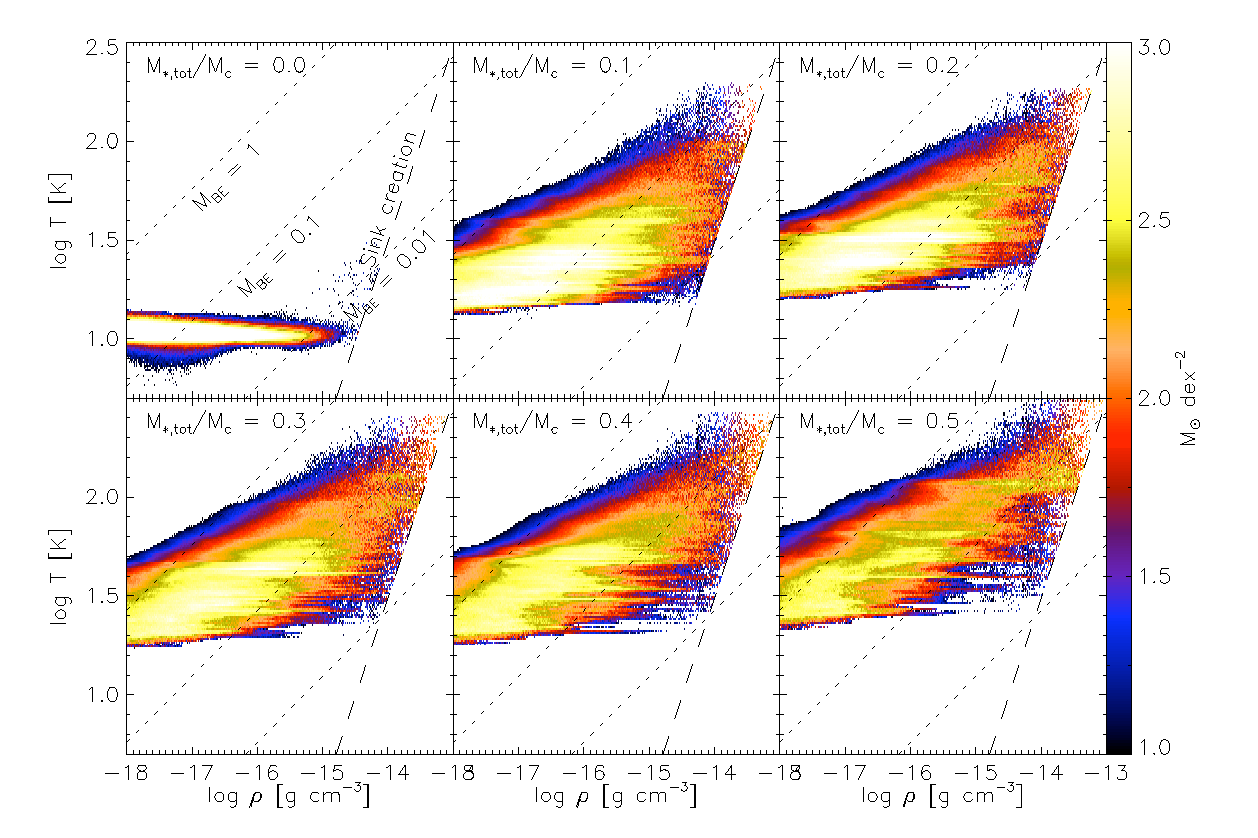
\includegraphics[width=\linewidth]{rhot_krumholz11}
\caption[Density-temperature distribution from a simulation of the formation of the ONC]{
\label{fig:rhot_krumholz11}
Density-temperature distributions measured from a simulation of the formation of an ONC-like star cluster, including radiative transfer and stellar feedback \citep{krumholz11c}. The panels show the distribution at different times in the simulation, characterized by the fraction of mass that has been turned into stars. Doted lines show lines of constant Bonnor-Ebert mass (in $M_\odot$), while dashed lines show the threshold for sink particle formation in the simulation.
}
\end{figure}

These two observations suggest that one can build a model for the IMF around radiative feedback. There are a few numerical and analytic papers that attempt to do so, including \citet{bate09a, bate12a}, \citet{krumholz11e}, \citet{krumholz12b}, and \citet{guszejnov16a}. The central idea for these models is that radiative feedback shuts off fragmentation at a characteristic mass scale that sets the peak of the IMF.

Suppose that we form a first, small protostellar that radiates at a rate $L$. The temperature of the material at a distance $R$ from it, assuming the gas is optically thick, will be roughly
\begin{equation}
L \approx 4 \pi \sigma_{\rm SB} R^2 T^4,
\end{equation}
where $\sigma_{\rm SB}$ is the Stefan-Boltzmann constant. Now let us compute the Bonnor-Ebert mass using the temperature $T$:
\begin{equation}
M_{\rm BE} \approx \frac{c_s^3}{\sqrt{G^3\rho}} = \sqrt{\left(\frac{k_B T}{\mu m_{\rm H} G}\right)^3 \frac{1}{\rho}},
\end{equation}
where $\mu=2.33$ is the mean particle mass, and we are omitting the factor of $1.18$ for simplicity. Note that $M_{\rm BE}$ here is a function of $R$. At small $R$, the temperature is large and thus $M_{\rm BE}$ is large, while at larger distances the gas is cooler and $M_{\rm BE}$ falls.

Now let us compare this mass to the mass enclosed within the radius $R$, which is $M=(4/3)\pi R^3 \rho$. At small radii, $M_{\rm BE}$ greatly exceeds the enclosed mass, while at large radii $M_{\rm BE}$ is much less than the enclosed mass. A reasonable hypothesis is that fragmentation will be suppressed out to the point where $M \approx M_{\rm BE}$. If we solve for the radius $R$ and mass $M$ at which this condition is met, we obtain
\begin{equation}
M  \approx \left(\frac{1}{36\pi}\right)^{1/10} \left(\frac{k_B}{G \mu m_{\rm H}}\right)^{6/5} \left(\frac{L}{\sigma_{\rm SB}}\right)^{3/10} \rho^{-1/5}.
\end{equation}

To go further, we need to know the luminosity $L$. The good news is that, for reasons to be discussed in Chapter \ref{ch:protostar_evol}, the luminosity is dominated by accretion, and the energy produced by accretion is simply the accretion rate multiplied by a roughly fixed energy yield per unit mass. In other words, we can write
\begin{equation}
L \approx \psi \dot{M},
\end{equation}
where $\psi \approx 10^{14}$ erg g$^{-1}$, and can in fact be written in terms of fundamental constants. Taking this on faith for now, if we further assume that stars form over a time of order a free-fall time, then
\begin{equation}
\dot{M} \approx M \sqrt{G\rho},
\end{equation}
and substituting this into the equation for $M$ above and solving gives
\begin{eqnarray}
M & \approx & \left(\frac{1}{36\pi}\right)^{1/7} \left(\frac{k_B}{G \mu m_{\rm H}}\right)^{12/7} \left(\frac{\psi}{\sigma_{\rm SB}}\right)^{3/7} \rho^{-1/14} \\
& = & 0.3 \left(\frac{n}{100\mbox{ cm}^{-3}}\right)^{-1/14} M_\odot,
\end{eqnarray}
where $n = \rho/(\mu m_{\rm H})$. Thus we get a characteristic mass that is a good match to the IMF peak, and that depends only very, very weaky on the ambient density.

Simulations including radiation seem to support the idea that this effect can pick out a characteristic peak ISM mass. The main downside to this hypothesis is that it has little to say by itself about the powerlaw tail of the IMF. This is not so much a problem with the model as an omission, and a promising area of research seems to be joining a non-isothermal model such as this onto a turbulent fragmentation or competitive accretion model to explain the full IMF.

